\documentclass[tikz,border=5pt]{standalone}
\usepackage{amsmath}
\usepackage{braket}
\usetikzlibrary{arrows.meta, calc, decorations.markings}

\begin{document}
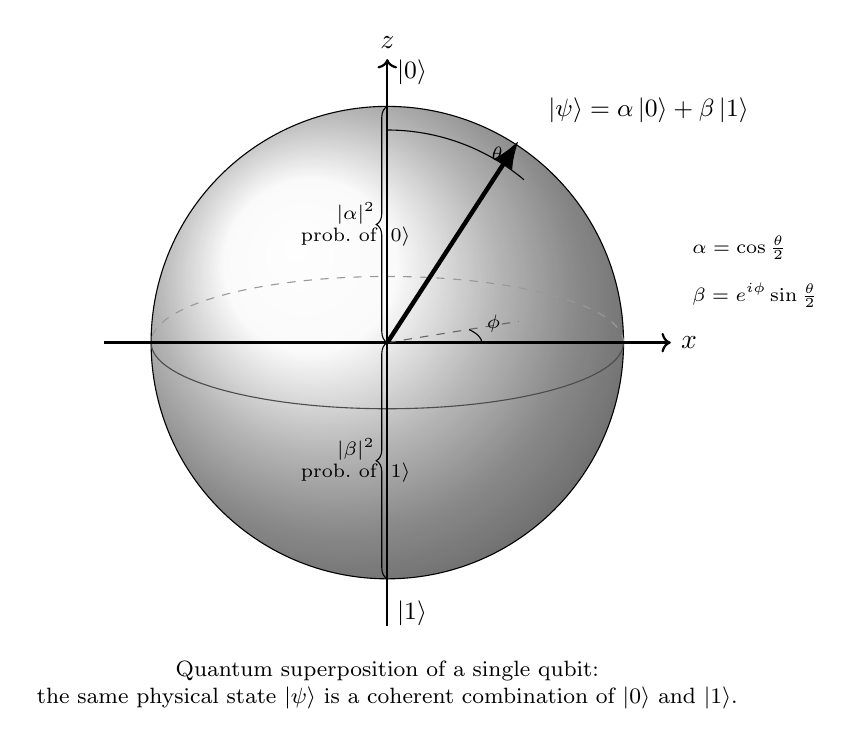
\begin{tikzpicture}[scale=3,
   axis/.style={->, thick},
   basislabel/.style={anchor=south east, inner sep=1pt, font=\small},
   statelabel/.style={anchor=west, font=\small},
   myvec/.style={-Latex, thick},
]

% Bloch sphere
\shade[ball color=white!95!gray, opacity=0.9] (0,0) circle (1cm);
\draw[thin, black] (0,0) circle (1cm);

% Draw "equator" ellipse (x-y plane)
\draw[thin, black!70] (-1,0) arc[start angle=180, end angle=360, x radius=1cm, y radius=0.28cm];
\draw[dashed, thin, black!40] (1,0) arc[start angle=0, end angle=180, x radius=1cm, y radius=0.28cm];

% Axes
\draw[axis] (0,-1.2) -- (0,1.2) node[above] {$z$};
\draw[axis] (-1.2,0) -- (1.2,0) node[right] {$x$};

% Poles: |0> at +z, |1> at -z
\node[font=\small, anchor=south west] at (0,1.05) {$\ket{0}$};
\node[font=\small, anchor=north west] at (0,-1.05) {$\ket{1}$};

% State vector |ψ>
% We'll pick some angles θ and φ.
% θ = polar angle from +z, φ = azimuth in x-y plane.
% Say θ = 40°, φ = 30°
\pgfmathsetmacro{\th}{40}   % polar
\pgfmathsetmacro{\ph}{30}   % azimuth
\pgfmathsetmacro{\xp}{sin(\th)*cos(\ph)}
\pgfmathsetmacro{\yp}{0.28*sin(\th)*sin(\ph)} % projected y (ellipse scaling)
\pgfmathsetmacro{\zp}{cos(\th)}

% draw projection of state onto equator
\draw[dashed, black!60] (0,0) -- (\xp,\yp);

% state vector
\draw[myvec, ultra thick] (0,0) -- (\xp,\yp+\zp);

% angle θ from +z axis
\draw[thin] (0,0.9) arc[start angle=90, end angle={90-\th}, radius=0.9cm];
\node[font=\scriptsize, anchor=west] at (0.4,0.8) {$\theta$};

% angle φ in x-y plane
\draw[thin] (0.4,0) arc[start angle=0, end angle=\ph, x radius=0.4cm, y radius=0.11cm];
\node[font=\scriptsize, anchor=west] at (0.38,0.08) {$\phi$};

% Label the state vector
\node[statelabel] at ($(0,0)!1.15!(\xp,\yp+\zp)$) {$\ket{\psi} =
\alpha\ket{0} + \beta\ket{1}$};

% Show alpha,beta magnitudes as cos(θ/2), sin(θ/2)
\node[font=\scriptsize, align=left, anchor=west] at (1.25,0.4) {$\alpha = \cos\frac{\theta}{2}$};
\node[font=\scriptsize, align=left, anchor=west] at (1.25,0.2) {$\beta = e^{i\phi}\sin\frac{\theta}{2}$};

% Little braces showing probabilities
\draw[decorate,decoration={brace, amplitude=4pt}]
 (0,0) -- (0,1)
 node[midway, xshift=-0.4cm, font=\scriptsize, align=center]
 {$|\alpha|^2$\\prob.\ of $\ket{0}$};

\draw[decorate,decoration={brace, amplitude=4pt}]
 (0,-1) -- (0,0)
 node[midway, xshift=-0.4cm, font=\scriptsize, align=center]
 {$|\beta|^2$\\prob.\ of $\ket{1}$};

% Caption under figure
\node[font=\footnotesize, align=center] at (0,-1.45)
{Quantum superposition of a single qubit:\\
the same physical state $\ket{\psi}$ is a coherent combination
of $\ket{0}$ and $\ket{1}$.};

\end{tikzpicture}
\end{document}
